% Greedy Algorithms Part 1 -- Metropolis beamer slides
% Compile: pdflatex greedy-1.tex (x2)
\documentclass[10pt,aspectratio=169]{beamer}

\usetheme{metropolis}
\metroset{block=fill, numbering=fraction, progressbar=frametitle}

\usepackage[T1]{fontenc}
\usepackage{amsmath, amssymb}
\usepackage{listings}
\usepackage{booktabs}
\usepackage{tikz}
\usepackage{pgfplots}
\pgfplotsset{compat=1.18}
\usetikzlibrary{arrows.meta, positioning, decorations.pathreplacing, calc}

% ---- colors -------------------------------------------------------------
\definecolor{mLightBlue}{HTML}{4C72B0}
\definecolor{mGreen}{HTML}{55A868}
\definecolor{mRed}{HTML}{C44E52}
\definecolor{mGray}{HTML}{BFBFBF}
\setbeamercolor{alerted text}{fg=mRed}

% ---- code style ---------------------------------------------------------
\lstdefinestyle{jl}{
  basicstyle=\ttfamily\footnotesize,
  keywordstyle=\color{mRed}\bfseries,
  commentstyle=\color{mGreen}\itshape,
  numberstyle=\tiny\color{mGray},
  showstringspaces=false,
  breaklines=true,
  columns=fullflexible,
  morekeywords={function,for,in,if,else,elseif,end,return,length,while}
}
\lstset{style=jl}

% ---- tree helpers -------------------------------------------------------
\tikzset{
  hnode/.style={draw, circle, minimum size=7.5mm, inner sep=0pt,
                fill=mLightBlue!20, font=\small},
  hleaf/.style={draw, rounded corners, minimum size=7.5mm, inner sep=2pt,
                fill=mGreen!30, font=\small},
  hedge/.style={mGray, thick},
}

% ---- title --------------------------------------------------------------
\title{Greedy Algorithms, Part 1}
\subtitle{Files on Tape, Huffman Coding}
\date{}
\author{}

\begin{document}

\maketitle

% =========================================================================
\begin{frame}{Greedy Algorithms}
  Build a solution through a series of steps, each of which takes the choice
  that looks best \alert{right now}.

  \bigskip
  \pause

  \begin{center}
  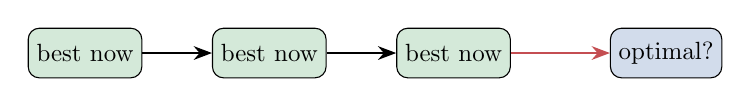
\begin{tikzpicture}[scale=0.9, every node/.style={transform shape}]
    \node[draw, rounded corners, fill=mGreen!25, minimum height=7mm] (a) at (0,0) {best now};
    \node[draw, rounded corners, fill=mGreen!25, minimum height=7mm] (b) at (2.6,0) {best now};
    \node[draw, rounded corners, fill=mGreen!25, minimum height=7mm] (c) at (5.2,0) {best now};
    \node[draw, rounded corners, fill=mLightBlue!25, minimum height=7mm] (d) at (8.2,0) {optimal?};
    \draw[-{Stealth}, thick] (a) -- (b);
    \draw[-{Stealth}, thick] (b) -- (c);
    \draw[-{Stealth}, thick, mRed] (c) -- (d);
  \end{tikzpicture}
  \end{center}

  \bigskip
  \pause
  \begin{center}
    The hard part is never the algorithm. It is proving the local choice is
    globally optimal.
  \end{center}
\end{frame}

% =========================================================================
\section{Storing Files on Tape}

\begin{frame}{The Problem}
  $n$ files with sizes $s_1, \ldots, s_n$ sit on a tape. Tape access is
  \alert{sequential}: reading a file means reading everything before it first.

  \bigskip
  \begin{center}
  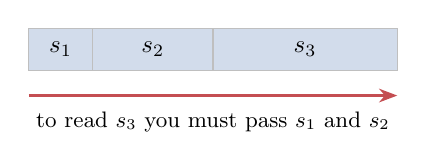
\begin{tikzpicture}[scale=0.9, every node/.style={transform shape}]
    \foreach \w/\lbl/\x [count=\i] in {0.9/$s_1$/0, 1.7/$s_2$/0.9, 2.6/$s_3$/2.6} {
      \fill[mLightBlue!25] (\x,0) rectangle ++(\w,0.6);
      \draw[mGray] (\x,0) rectangle ++(\w,0.6);
      \node at ({\x+\w/2},0.3) {\lbl};
    }
    \draw[-{Stealth}, thick, mRed] (0,-0.35) -- (5.2,-0.35);
    \node[below] at (2.6,-0.45) {\small to read $s_3$ you must pass $s_1$ and $s_2$};
  \end{tikzpicture}
  \end{center}

  \bigskip
  If the files are stored in order $\sigma$, the cost of retrieving
  $\sigma(j)$ is
  \[
    \text{cost}(\sigma(j)) = \sum_{k=1}^{j} s_{\sigma(k)}.
  \]
\end{frame}

\begin{frame}{Order Matters}
  Three files with sizes $[1, 2, 3]$.

  \bigskip
  \begin{center}
  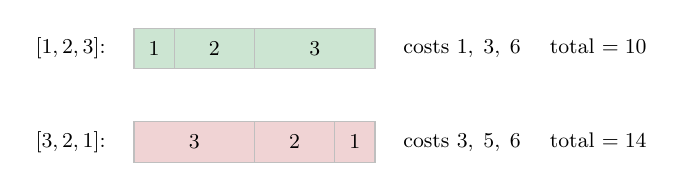
\begin{tikzpicture}[scale=0.85, every node/.style={transform shape}]
    % order 1,2,3
    \node[left] at (-0.3,0.3) {\small $[1,2,3]$:};
    \foreach \w/\lbl/\x in {0.6/1/0, 1.2/2/0.6, 1.8/3/1.8} {
      \fill[mGreen!30] (\x,0) rectangle ++(\w,0.6);
      \draw[mGray] (\x,0) rectangle ++(\w,0.6);
      \node at ({\x+\w/2},0.3) {\small \lbl};
    }
    \node[right] at (3.9,0.3) {\small costs $1,\; 3,\; 6$ \quad total $= \alert{10}$};
    % order 3,2,1
    \node[left] at (-0.3,-1.1) {\small $[3,2,1]$:};
    \foreach \w/\lbl/\x in {1.8/3/0, 1.2/2/1.8, 0.6/1/3.0} {
      \fill[mRed!25] (\x,-1.4) rectangle ++(\w,0.6);
      \draw[mGray] (\x,-1.4) rectangle ++(\w,0.6);
      \node at ({\x+\w/2},-1.1) {\small \lbl};
    }
    \node[right] at (3.9,-1.1) {\small costs $3,\; 5,\; 6$ \quad total $= \alert{14}$};
  \end{tikzpicture}
  \end{center}

  \bigskip
  \begin{center}
    Same files, different total cost. Which order is best?
  \end{center}
\end{frame}

\begin{frame}{Total Retrieval Cost}
  Assuming every file is equally likely to be requested,
  \[
    C(\sigma) \;=\; \sum_{j=1}^{n} \sum_{k=1}^{j} s_{\sigma(k)}
              \;=\; \sum_{j=1}^{n} (n - j + 1)\, s_{\sigma(j)}.
  \]

  \pause
  \bigskip
  Why the second form? File $\sigma(j)$ is read for its own retrieval and for
  every file after it:

  \begin{center}
  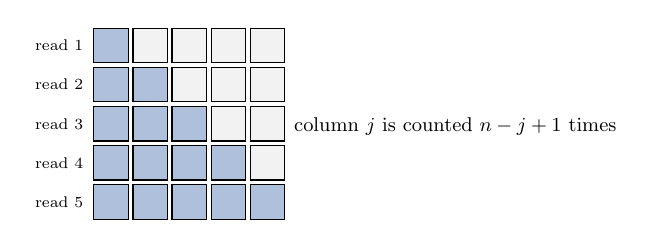
\begin{tikzpicture}[scale=0.8, every node/.style={transform shape}]
    \foreach \i in {1,...,5} {
      \foreach \k in {1,...,5} {
        \ifnum\k<\i \def\fc{mLightBlue!45}\else\def\fc{black!5}\fi
        \ifnum\k=\i \def\fc{mLightBlue!45}\fi
        \node[draw, fill=\fc, minimum size=5.5mm] at (\k*0.62, -\i*0.62) {};
      }
      \node[left] at (0.3, -\i*0.62) {\scriptsize read \i};
    }
    \node[right] at (3.4,-1.9) {\small column $j$ is counted $n-j+1$ times};
  \end{tikzpicture}
  \end{center}
\end{frame}

\begin{frame}{The Greedy Rule}
  \begin{block}{Claim}
    Sorting the files in \alert{non-decreasing order of size} is optimal.
  \end{block}

  \bigskip
  \textbf{Intuition.} A file placed early adds its size to the cost of every
  later retrieval. So the ones we pay for most often should be the
  \alert{small} ones.

  \bigskip
  \begin{center}
    The rule is obvious. The proof is the interesting part.
  \end{center}
\end{frame}

\begin{frame}{Exchange Argument}
  Suppose an optimal order has adjacent files $a$ then $b$ with
  $s_a > s_b$. Swap them.

  \bigskip
  \begin{center}
  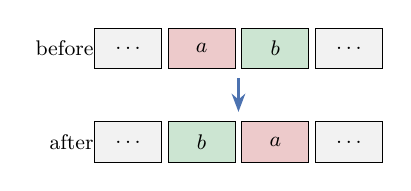
\begin{tikzpicture}[scale=0.85, every node/.style={transform shape}]
    % before
    \node[left] at (-0.3,0.3) {\small before:};
    \foreach \lbl/\x/\fc in {$\ldots$/0/black!5, $a$/1.1/mRed!30, $b$/2.2/mGreen!30, $\ldots$/3.3/black!5} {
      \node[draw, minimum width=10mm, minimum height=6mm, fill=\fc] at (\x,0.3) {\small \lbl};
    }
    % after
    \node[left] at (-0.3,-1.1) {\small after:};
    \foreach \lbl/\x/\fc in {$\ldots$/0/black!5, $b$/1.1/mGreen!30, $a$/2.2/mRed!30, $\ldots$/3.3/black!5} {
      \node[draw, minimum width=10mm, minimum height=6mm, fill=\fc] at (\x,-1.1) {\small \lbl};
    }
    \draw[-{Stealth}, thick, mLightBlue] (1.65,-0.15) -- (1.65,-0.65);
  \end{tikzpicture}
  \end{center}

  \pause
  \bigskip
  \begin{itemize}
    \item Reading $a$ costs $s_b$ \alert{more} (now $b$ comes first).
    \item Reading $b$ costs $s_a$ \alert{less} (it no longer skips $a$).
    \item Every other file is unaffected.
  \end{itemize}
\end{frame}

\begin{frame}{Exchange Argument}
  The net change in total cost is
  \[
    s_b - s_a \;<\; 0 \qquad \text{whenever } s_b < s_a .
  \]

  \bigskip
  So the swap \alert{strictly improves} the order, contradicting optimality.

  \bigskip
  Hence no optimal order has a larger file immediately before a smaller one,
  which means the optimal order is sorted by non-decreasing size.

  \bigskip
  \begin{alertblock}{}
    Sorting dominates: $O(n \log n)$.
  \end{alertblock}
\end{frame}

% =========================================================================
\section{Files with Access Probabilities}

\begin{frame}{A Twist}
  Now file $i$ also has an access probability $p_i > 0$, with
  $\sum_i p_i = 1$. The \alert{expected} retrieval cost is
  \[
    C(\sigma) = \sum_{j=1}^{n} p_{\sigma(j)} \sum_{k=1}^{j} s_{\sigma(k)}.
  \]

  \pause
  \bigskip
  \textbf{Example.} $(s_1, p_1) = (10,\, 0.1)$ and $(s_2, p_2) = (1,\, 0.9)$.

  \bigskip
  \begin{center}
  \begin{tabular}{lll}
    \toprule
    order & expected cost & \\
    \midrule
    $[1,2]$ & $0.1 \cdot 10 + 0.9 \cdot (10+1)$ & $= 10.9$ \\
    $[2,1]$ & $0.9 \cdot 1 \; + 0.1 \cdot (1+10)$ & $= \alert{2.0}$ \\
    \bottomrule
  \end{tabular}
  \end{center}

  \bigskip
  \begin{center}
    File $1$ is \emph{bigger}, but file $2$ is asked for far more often.
  \end{center}
\end{frame}

\begin{frame}{The Greedy Rule}
  \begin{block}{Claim}
    Sorting by \alert{non-decreasing $s_i / p_i$} is optimal.
  \end{block}

  \bigskip
  \begin{center}
  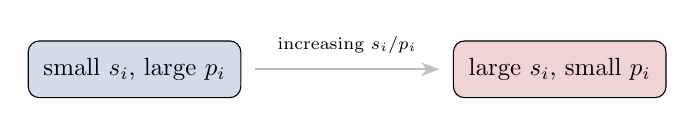
\begin{tikzpicture}[scale=0.9, every node/.style={transform shape}]
    \node[draw, rounded corners, fill=mLightBlue!25, minimum height=8mm, minimum width=30mm] (a) at (0,0) {small $s_i$, large $p_i$};
    \node[draw, rounded corners, fill=mRed!25, minimum height=8mm, minimum width=30mm] (b) at (6,0) {large $s_i$, small $p_i$};
    \draw[-{Stealth}, thick, mGray] (1.7,0) -- (4.3,0);
    \node[above] at (3,0.1) {\scriptsize increasing $s_i/p_i$};
  \end{tikzpicture}
  \end{center}

  \bigskip
  \begin{center}
    Sorting by size alone, or by probability alone, is not enough.
    The \alert{ratio} is what matters.
  \end{center}
\end{frame}

\begin{frame}{Exchange Argument}
  Suppose adjacent files $a$ then $b$ have
  $\dfrac{s_a}{p_a} > \dfrac{s_b}{p_b}$. First rewrite that:
  \[
    \frac{s_a}{p_a} > \frac{s_b}{p_b}
    \;\Longrightarrow\;
    p_b s_a > p_a s_b
    \;\Longrightarrow\;
    \alert{p_a s_b - p_b s_a < 0}.
  \]

  \pause
  \bigskip
  Now swap $a$ and $b$:
  \begin{itemize}
    \item reading $a$ costs $s_b$ more, contributing $+\, p_a s_b$;
    \item reading $b$ costs $s_a$ less, contributing $-\, p_b s_a$;
    \item everything else is unaffected.
  \end{itemize}

  \pause
  \bigskip
  The net change is $p_a s_b - p_b s_a < 0$, contradicting optimality.
  Again $O(n \log n)$.
\end{frame}

% =========================================================================
\section{Huffman Coding}

\begin{frame}{Prefix Trees}
  A \alert{prefix tree} is a full binary tree whose leaves are the symbols.
  Read the codeword off the root-to-leaf path: left is \texttt{0}, right is
  \texttt{1}.

  \bigskip
  \begin{center}
  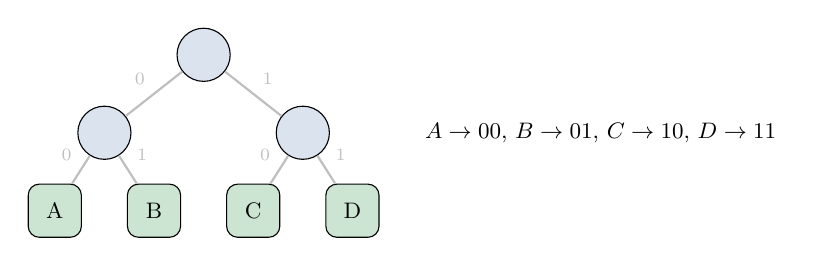
\begin{tikzpicture}[scale=0.9, every node/.style={transform shape}]
    \node[hnode] (r) at (0,0) {};
    \node[hnode] (l) at (-1.4,-1.1) {};
    \node[hnode] (rr) at (1.4,-1.1) {};
    \node[hleaf] (A) at (-2.1,-2.2) {A};
    \node[hleaf] (B) at (-0.7,-2.2) {B};
    \node[hleaf] (C) at (0.7,-2.2) {C};
    \node[hleaf] (D) at (2.1,-2.2) {D};
    \draw[hedge] (r) -- node[above left, font=\scriptsize] {0} (l);
    \draw[hedge] (r) -- node[above right, font=\scriptsize] {1} (rr);
    \draw[hedge] (l) -- node[above left, font=\scriptsize] {0} (A);
    \draw[hedge] (l) -- node[above right, font=\scriptsize] {1} (B);
    \draw[hedge] (rr) -- node[above left, font=\scriptsize] {0} (C);
    \draw[hedge] (rr) -- node[above right, font=\scriptsize] {1} (D);
    \node[right] at (3.0,-1.1) {\small $A \to 00$, $B \to 01$, $C \to 10$, $D \to 11$};
  \end{tikzpicture}
  \end{center}

  \bigskip
  \begin{center}
    This one is just fixed-length encoding, $2$ bits per symbol.
  \end{center}
\end{frame}

\begin{frame}{Prefix-Free, for Free}
  \begin{block}{Property}
    No codeword is a prefix of another.
  \end{block}

  \bigskip
  Why it holds automatically: if $x$'s codeword were a prefix of $y$'s, then
  $x$ would lie \alert{on the path} to $y$, making $x$ an internal node.

  \bigskip
  But every symbol is a \alert{leaf}. Contradiction.

  \bigskip
  \begin{center}
    This is exactly what makes decoding unambiguous.
  \end{center}
\end{frame}

\begin{frame}{Variable Length Can Do Better}
  If some symbols are much more frequent, give them shorter codewords.

  \bigskip
  \begin{center}
  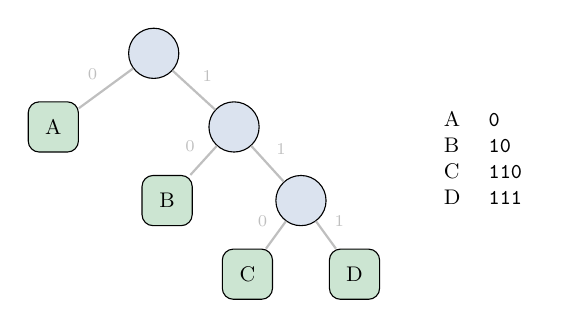
\begin{tikzpicture}[scale=0.85, every node/.style={transform shape}]
    \node[hnode] (r)  at (0,0) {};
    \node[hleaf] (A)  at (-1.5,-1.1) {A};
    \node[hnode] (n1) at (1.2,-1.1) {};
    \node[hleaf] (B)  at (0.2,-2.2) {B};
    \node[hnode] (n2) at (2.2,-2.2) {};
    \node[hleaf] (C)  at (1.4,-3.3) {C};
    \node[hleaf] (D)  at (3.0,-3.3) {D};
    \draw[hedge] (r)  -- node[above left, font=\scriptsize] {0} (A);
    \draw[hedge] (r)  -- node[above right, font=\scriptsize] {1} (n1);
    \draw[hedge] (n1) -- node[above left, font=\scriptsize] {0} (B);
    \draw[hedge] (n1) -- node[above right, font=\scriptsize] {1} (n2);
    \draw[hedge] (n2) -- node[above left, font=\scriptsize] {0} (C);
    \draw[hedge] (n2) -- node[above right, font=\scriptsize] {1} (D);
    \node[right] at (4.0,-1.6) {\small
      \begin{tabular}{ll}
        A & \texttt{0} \\
        B & \texttt{10} \\
        C & \texttt{110} \\
        D & \texttt{111} \\
      \end{tabular}};
  \end{tikzpicture}
  \end{center}

  \bigskip
  \begin{center}
    \texttt{AABABCD}: fixed length needs $7 \times 2 = 14$ bits,\\
    this tree needs $1{+}1{+}2{+}1{+}2{+}3{+}3 = \alert{13}$ bits.
  \end{center}
\end{frame}

\begin{frame}{Cost of a Prefix Tree}
  With symbols $1, \ldots, n$ of frequencies $f_1, \ldots, f_n$,

  \begin{alertblock}{}
    \[
      \text{cost}(T) = \sum_{i=1}^{n} f_i \cdot d_T(i)
    \]
  \end{alertblock}

  \bigskip
  where $d_T(i)$ is the depth of leaf $i$, that is the length of symbol $i$'s
  codeword.

  \bigskip
  \begin{center}
    \textbf{Goal:} find the tree $T$ of minimum cost.
  \end{center}
\end{frame}

\begin{frame}{Huffman's Algorithm}
  The greedy idea: \alert{rare symbols get long codewords}. Build the tree
  \alert{bottom up}.

  \bigskip
  \begin{enumerate}
    \item Make a leaf for each symbol $i$ with key $f_i$; put them all in a
          min-heap.
    \bigskip
    \item While the heap has more than one node:
      \begin{itemize}
        \item[] extract the two smallest, $u$ and $v$;
        \item[] create $w$ with $f_w = f_u + f_v$ and children $u, v$;
        \item[] insert $w$ back.
      \end{itemize}
    \bigskip
    \item The last remaining node is the root.
  \end{enumerate}

  \bigskip
  \begin{center}
    $n-1$ merges, each $O(\log n)$, so $O(n \log n)$.
  \end{center}
\end{frame}

% ---------------------------------------------------------------- example
\begin{frame}{Worked Example}
  \begin{center}
  \begin{tabular}{lccccc}
    \toprule
    Symbol & A & B & C & D & E \\
    \midrule
    Freq   & 45 & 13 & 12 & 16 & 9 \\
    \bottomrule
  \end{tabular}
  \end{center}

  \bigskip
  \begin{center}
  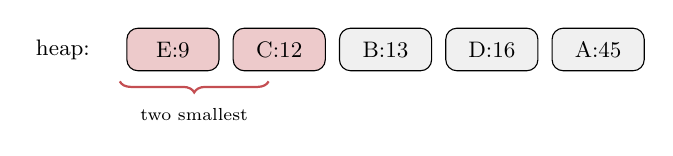
\begin{tikzpicture}[scale=0.9, every node/.style={transform shape}]
    \node[left] at (-1.05,0) {\small heap:};
    \foreach \lbl/\i in {{E:9}/0, {C:12}/1, {B:13}/2, {D:16}/3, {A:45}/4} {
      \ifnum\i<2 \def\fc{mRed!30}\else\def\fc{black!6}\fi
      \node[draw, rounded corners, minimum width=13mm, minimum height=6mm,
            fill=\fc] at (\i*1.5,0) {\small \lbl};
    }
    \draw[decorate, decoration={brace, amplitude=4pt}, mRed, thick]
      (1.35,-0.45) -- (-0.75,-0.45);
    \node[below] at (0.3,-0.7) {\scriptsize two smallest};
  \end{tikzpicture}
  \end{center}
\end{frame}

\begin{frame}{Merging}
  \begin{center}
  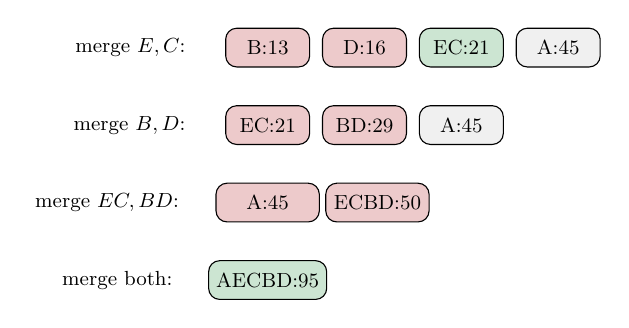
\begin{tikzpicture}[scale=0.82, every node/.style={transform shape}]
    % step 1
    \node[left] at (-1.15,0) {\small merge $E, C$:};
    \foreach \lbl/\i/\fc in {{B:13}/0/mRed!30, {D:16}/1/mRed!30, {EC:21}/2/mGreen!30, {A:45}/3/black!6}
      \node[draw, rounded corners, minimum width=13mm, minimum height=6mm, fill=\fc] at (\i*1.5,0) {\small \lbl};
    % step 2
    \node[left] at (-1.15,-1.2) {\small merge $B, D$:};
    \foreach \lbl/\i/\fc in {{EC:21}/0/mRed!30, {BD:29}/1/mRed!30, {A:45}/2/black!6}
      \node[draw, rounded corners, minimum width=13mm, minimum height=6mm, fill=\fc] at (\i*1.5,-1.2) {\small \lbl};
    % step 3
    \node[left] at (-1.25,-2.4) {\small merge $EC, BD$:};
    \foreach \lbl/\i/\fc in {{A:45}/0/mRed!30, {ECBD:50}/1/mRed!30}
      \node[draw, rounded corners, minimum width=16mm, minimum height=6mm, fill=\fc] at (\i*1.7,-2.4) {\small \lbl};
    % step 4
    \node[left] at (-1.35,-3.6) {\small merge both:};
    \node[draw, rounded corners, minimum width=18mm, minimum height=6mm, fill=mGreen!30] at (0,-3.6) {\small AECBD:95};
  \end{tikzpicture}
  \end{center}

  \bigskip
  \begin{center}
    \small Red marks the two nodes pulled off the heap at each step.
  \end{center}
\end{frame}

\begin{frame}{The Resulting Tree}
  \begin{center}
  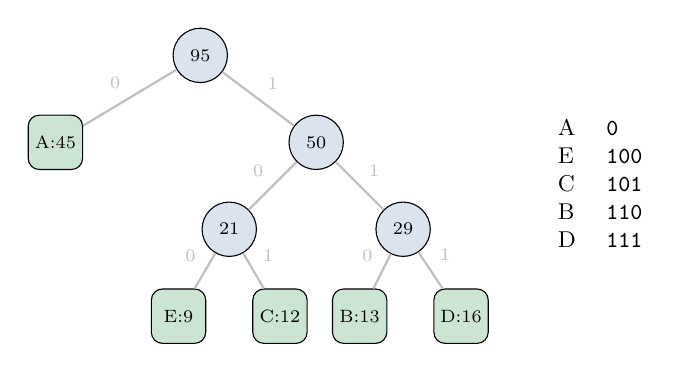
\begin{tikzpicture}[scale=0.92, every node/.style={transform shape}]
    \node[hnode] (r)  at (0,0) {\scriptsize 95};
    \node[hleaf] (A)  at (-2.0,-1.2) {\scriptsize A:45};
    \node[hnode] (n1) at (1.6,-1.2) {\scriptsize 50};
    \node[hnode] (n2) at (0.4,-2.4) {\scriptsize 21};
    \node[hnode] (n3) at (2.8,-2.4) {\scriptsize 29};
    \node[hleaf] (E)  at (-0.3,-3.6) {\scriptsize E:9};
    \node[hleaf] (C)  at (1.1,-3.6) {\scriptsize C:12};
    \node[hleaf] (B)  at (2.2,-3.6) {\scriptsize B:13};
    \node[hleaf] (D)  at (3.6,-3.6) {\scriptsize D:16};
    \draw[hedge] (r)  -- node[above left,  font=\scriptsize] {0} (A);
    \draw[hedge] (r)  -- node[above right, font=\scriptsize] {1} (n1);
    \draw[hedge] (n1) -- node[above left,  font=\scriptsize] {0} (n2);
    \draw[hedge] (n1) -- node[above right, font=\scriptsize] {1} (n3);
    \draw[hedge] (n2) -- node[above left,  font=\scriptsize] {0} (E);
    \draw[hedge] (n2) -- node[above right, font=\scriptsize] {1} (C);
    \draw[hedge] (n3) -- node[above left,  font=\scriptsize] {0} (B);
    \draw[hedge] (n3) -- node[above right, font=\scriptsize] {1} (D);
    \node[right] at (4.6,-1.8) {\small
      \begin{tabular}{ll}
        A & \texttt{0} \\
        E & \texttt{100} \\
        C & \texttt{101} \\
        B & \texttt{110} \\
        D & \texttt{111} \\
      \end{tabular}};
  \end{tikzpicture}
  \end{center}
\end{frame}

\begin{frame}{What It Saves}
  \[
    \text{cost}(T) = 45{\cdot}1 + 9{\cdot}3 + 12{\cdot}3 + 13{\cdot}3 + 16{\cdot}3
                   = \alert{195} \text{ bits}.
  \]

  \bigskip
  A fixed-length code needs $\lceil \log_2 5 \rceil = 3$ bits per symbol:
  \[
    3 \times 95 = 285 \text{ bits}.
  \]

  \bigskip
  \begin{center}
  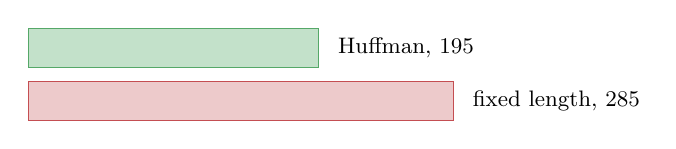
\begin{tikzpicture}[scale=0.9, every node/.style={transform shape}]
    \fill[mGreen!35, draw=mGreen] (0,0.4) rectangle (4.1,0.95);
    \node[right] at (4.25,0.675) {\small Huffman, $195$};
    \fill[mRed!30, draw=mRed] (0,-0.35) rectangle (6.0,0.2);
    \node[right] at (6.15,-0.075) {\small fixed length, $285$};
  \end{tikzpicture}
  \end{center}

  \bigskip
  \begin{center}
    \small The more skewed the frequencies, the bigger the win.
  \end{center}
\end{frame}

\begin{frame}{Encoding and Decoding}
  \textbf{Encoding} is a table lookup and concatenation:
  \[
    \texttt{A B C A D E} \;\longrightarrow\;
    \texttt{0} \cdot \texttt{110} \cdot \texttt{101} \cdot \texttt{0}
    \cdot \texttt{111} \cdot \texttt{100}
    \;=\; \texttt{01101010111100}
  \]

  \pause
  \bigskip
  \textbf{Decoding} walks the tree. Start at the root, follow \texttt{0} left
  and \texttt{1} right; on reaching a leaf, emit the symbol and return to the
  root.

  \bigskip
  \begin{center}
  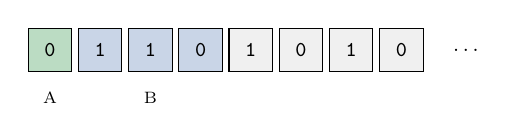
\begin{tikzpicture}[scale=0.85, every node/.style={transform shape}]
    \foreach \b/\i/\fc in {0/0/mGreen!40, 1/1/mLightBlue!30, 1/2/mLightBlue!30,
                           0/3/mLightBlue!30, 1/4/black!6, 0/5/black!6,
                           1/6/black!6, 0/7/black!6} {
      \node[draw, minimum size=6.5mm, fill=\fc] at (\i*0.75,0) {\small \tt \b};
    }
    \node[right] at (5.9,0) {\small $\ldots$};
    \node[below] at (0,-0.5) {\scriptsize A};
    \node[below] at (1.5,-0.5) {\scriptsize B};
  \end{tikzpicture}
  \end{center}

  \bigskip
  \begin{center}
    \small Prefix-freeness is what makes this walk unambiguous.
  \end{center}
\end{frame}

% ---------------------------------------------------------------- exercise
\begin{frame}{Exercise}
  \begin{center}
    Build the Huffman tree for these frequencies and give the total cost.
  \end{center}

  \bigskip
  \begin{center}
  \begin{tabular}{lcccc}
    \toprule
    Symbol & A & B & C & D \\
    \midrule
    Freq   & 5 & 2 & 1 & 1 \\
    \bottomrule
  \end{tabular}
  \end{center}

  \bigskip
  \begin{center}
    \small Compare it against a fixed-length code.
  \end{center}
\end{frame}

\begin{frame}{Solution}
  Merge $C{:}1$ and $D{:}1$ into $CD{:}2$, then $B{:}2$ with $CD{:}2$ into $4$,
  then $A{:}5$ with that into $9$.

  \begin{center}
  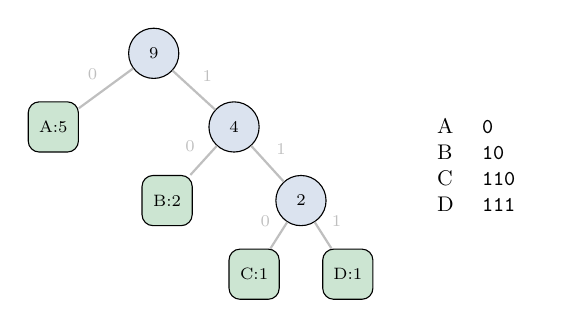
\begin{tikzpicture}[scale=0.85, every node/.style={transform shape}]
    \node[hnode] (r)  at (0,0) {\scriptsize 9};
    \node[hleaf] (A)  at (-1.5,-1.1) {\scriptsize A:5};
    \node[hnode] (n1) at (1.2,-1.1) {\scriptsize 4};
    \node[hleaf] (B)  at (0.2,-2.2) {\scriptsize B:2};
    \node[hnode] (n2) at (2.2,-2.2) {\scriptsize 2};
    \node[hleaf] (C)  at (1.5,-3.3) {\scriptsize C:1};
    \node[hleaf] (D)  at (2.9,-3.3) {\scriptsize D:1};
    \draw[hedge] (r)  -- node[above left,  font=\scriptsize] {0} (A);
    \draw[hedge] (r)  -- node[above right, font=\scriptsize] {1} (n1);
    \draw[hedge] (n1) -- node[above left,  font=\scriptsize] {0} (B);
    \draw[hedge] (n1) -- node[above right, font=\scriptsize] {1} (n2);
    \draw[hedge] (n2) -- node[above left,  font=\scriptsize] {0} (C);
    \draw[hedge] (n2) -- node[above right, font=\scriptsize] {1} (D);
    \node[right] at (3.9,-1.7) {\small
      \begin{tabular}{ll}
        A & \texttt{0} \\
        B & \texttt{10} \\
        C & \texttt{110} \\
        D & \texttt{111} \\
      \end{tabular}};
  \end{tikzpicture}
  \end{center}

  \[
    \text{cost} = 5{\cdot}1 + 2{\cdot}2 + 1{\cdot}3 + 1{\cdot}3 = 15
    \quad\text{versus}\quad 2 \times 9 = 18 \text{ fixed length}.
  \]
\end{frame}

% ---------------------------------------------------------------- proof
\begin{frame}{Optimality: the Plan}
  Two steps.

  \bigskip
  \begin{enumerate}
    \item A \alert{structural lemma}: some optimal tree puts the two rarest
          symbols as siblings at maximum depth.
    \bigskip
    \item \alert{Induction} on $n$: merging those two and recursing is exactly
          what Huffman does.
  \end{enumerate}
\end{frame}

\begin{frame}{Sibling Lemma}
  \begin{block}{Lemma}
    Let $x, y$ be the two least frequent symbols. There is an optimal tree
    $T^\star$ in which $x$ and $y$ are \alert{siblings at maximum depth}.
  \end{block}

  \pause
  \bigskip
  \textbf{Proof.} Take any optimal $T^\star$ and let $a, b$ be siblings at
  maximum depth, with $f_a \le f_b$. Since $x, y$ are the two rarest,
  $f_x \le f_a$ and $f_y \le f_b$.

  \bigskip
  Swap $x$ with $a$. The cost changes by
  \[
    \big(f_x - f_a\big)\big(d_{T^\star}(a) - d_{T^\star}(x)\big) \;\le\; 0,
  \]
  since $f_x \le f_a$ and $a$ sits at maximum depth so
  $d_{T^\star}(a) \ge d_{T^\star}(x)$.
\end{frame}

\begin{frame}{Sibling Lemma}
  \begin{center}
  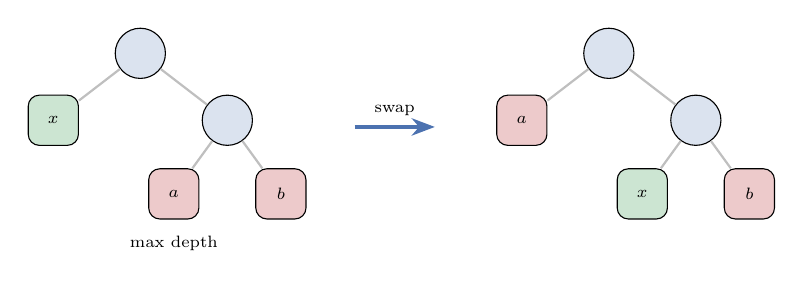
\begin{tikzpicture}[scale=0.85, every node/.style={transform shape}]
    % before
    \node[hnode] (r) at (0,0) {};
    \node[hleaf, fill=mGreen!30] (x) at (-1.3,-1.0) {\scriptsize $x$};
    \node[hnode] (w) at (1.3,-1.0) {};
    \node[hleaf, fill=mRed!30] (a) at (0.5,-2.1) {\scriptsize $a$};
    \node[hleaf, fill=mRed!30] (b) at (2.1,-2.1) {\scriptsize $b$};
    \draw[hedge] (r) -- (x); \draw[hedge] (r) -- (w);
    \draw[hedge] (w) -- (a); \draw[hedge] (w) -- (b);
    \node[below] at (0.5,-2.6) {\scriptsize max depth};
    % arrow
    \draw[-{Stealth}, very thick, mLightBlue] (3.2,-1.1) -- (4.4,-1.1);
    \node[above] at (3.8,-1.05) {\scriptsize swap};
    % after
    \begin{scope}[xshift=7cm]
      \node[hnode] (r2) at (0,0) {};
      \node[hleaf, fill=mRed!30] (a2) at (-1.3,-1.0) {\scriptsize $a$};
      \node[hnode] (w2) at (1.3,-1.0) {};
      \node[hleaf, fill=mGreen!30] (x2) at (0.5,-2.1) {\scriptsize $x$};
      \node[hleaf, fill=mRed!30] (b2) at (2.1,-2.1) {\scriptsize $b$};
      \draw[hedge] (r2) -- (a2); \draw[hedge] (r2) -- (w2);
      \draw[hedge] (w2) -- (x2); \draw[hedge] (w2) -- (b2);
    \end{scope}
  \end{tikzpicture}
  \end{center}

  \bigskip
  So $T'$ is no worse, hence also optimal. Swapping $y$ with $b$ the same way
  puts $x$ and $y$ together at maximum depth. $\square$
\end{frame}

\begin{frame}{Theorem}
  \begin{block}{}
    Huffman's algorithm produces an optimal prefix tree.
  \end{block}

  \bigskip
  \textbf{Base case.} $n = 2$: the only tree has both symbols at depth $1$,
  and that is what Huffman builds.

  \bigskip
  \textbf{Inductive step.} Assume optimality for $n-1$ symbols. Let $x, y$ be
  the two rarest. By the lemma, some optimal $T^\star$ has them as siblings
  under a node $w$, so
  \[
    d_{T^\star}(x) = d_{T^\star}(y) = d_{T^\star}(w) + 1.
  \]
\end{frame}

\begin{frame}{Theorem}
  Split the cost around $w$:
  \[
    \text{cost}(T^\star)
    = \sum_{i \ne x,y} f_i\, d_{T^\star}(i) + (f_x + f_y)\big(d_{T^\star}(w) + 1\big)
  \]
  \[
    = \underbrace{\left[ \sum_{i \ne x,y} f_i\, d_{T^\star}(i)
      + (f_x + f_y)\, d_{T^\star}(w) \right]}_{\text{cost}(T^\star_w)}
      \;+\; (f_x + f_y).
  \]

  \bigskip
  Here $T^\star_w$ is $T^\star$ with $x, y$ removed and $w$ made a leaf of
  frequency $f_x + f_y$: an instance with $n-1$ symbols.
\end{frame}

\begin{frame}{Theorem}
  Huffman does exactly this: merge $x$ and $y$ into $w$, recurse, then hang
  $x$ and $y$ back under $w$.

  \bigskip
  By the inductive hypothesis its tree $T_w$ on the reduced instance satisfies
  $\text{cost}(T_w) \le \text{cost}(T^\star_w)$. Therefore
  \[
    \text{cost}(T_H) = \text{cost}(T_w) + (f_x + f_y)
    \;\le\; \text{cost}(T^\star_w) + (f_x + f_y)
    = \text{cost}(T^\star).
  \]

  \bigskip
  \begin{center}
    Huffman's tree is at least as good as any optimal tree. $\blacksquare$
  \end{center}
\end{frame}

\end{document}
